\chapter{Establishment of laboratory methods and amalytical tools to assess genome-wide chromatin accessibility in clinical samples}
\label{ch:Results_1}


%%%%%%%%%%%%%%%%%%%%%%%%%%%%%%%%%%%%%%%%%%%%%%%%%%
\section{Introduction}
\subsection*{Previous and current methods to identify the accessible genome in cells and tissues}

\subsection*{Implementation of ATAC-seq to define the chromatin landscape}

\subsection*{Technical limitations and recent advances in optimisation}

Talk about ATAC being more variable, a native chromatin accessibility assessment without cross-linking. Role of transposase ability in accessing the chromatin, debri and DNA from dead cells adding noise

Paper to justify peak calling: A comparison of peak callers used for DNase-Seq data.

New ATAC but also explanations of the limitations: Characterization of chromatin accessibility with a transposome hypersensitive sites sequencing (THS-seq) assay

\subsection*{Challenges of working with clinical samples}

%%%%%%%%%%%%%%%%%%%%%%%%%%%%%%%%%%%%%%%%%%%%%%%%%%
\section{Results}
%

\subsection*{Establishment of an ATAC-seq data analysis pipeline based on current knowledge}
When the first ATAC-seq publication \parencite{Buenrostro2013} appeared, there were not well established protocols for the complete processing of the data. Since then, several publications have used ATAC-seq and modifications of this protocol together with a wide range of data analysis strategies to answer different biological questions. %Table summarising the main papers and approaches 

There are several limiting aspects in the process of analysing ATAC-seq data, including QC assessment, peak calling/filtering and differential analysis of chromatin accessibility regions between groups. Using the current knowledge in the field as well as on my own analysis, I agreed on the most appropriate criteria and parameters to implement in our in-house pipeline. For this purpose, I used ATAC data generated with the original protocol \parencite{Buenrostro2013} in paired CD14$^+$ monocytes and CD4$^+$ total T cells from the same three healthy individuals, all of them downsamples to 30 million of reads, in order to facilitate the comparison across all of them.

\subsubsection{Sample quality control}
Regarding QC measurements, the variability in performance of the methodology, particularly ATAC-seq and Fast-ATAC, has required to agree on few parameters to determine the quality of the samples before proceeding with downstream differential analysis. After reviewing the different read-outs implemented across different publications, I have identified the most informative ones showing supporting correlation between them.

Firstly, I analysed the fragment size distribution for each of the samples in order to determine if they recapitulate the expected nucleosome periodicity every $\sim$200bp. All the samples showed clear periodicity up to 600bp, clearly distinguishing chromatin organisation into mono-, di- and tri-nucleosomes. The relative intensity of nucleosome-free DNA fragments (<200pb) compared to nucleosome-bound DNA was greater for some of the samples (e.g CTL1 CD4$^+$ and CD14$^+$) and similar or lower for others (e.g CTL3 CD4$^+$ and CD14$^+$).


I analysed the enrichment over a random background of ATAC-seq reads across all the TSS for the identified Ensemble genes where nucleosome repositioning and an increase of chromatin accessibility take place to allow the transcriptional complex formation and initiation of transcription.


ATAC-seq signal intensity at the promoter of a constitutively expressed gene \textit{GAPDH}

Agreement between TSS enrichment values and the background levels in each of the samples.







\begin{figure}[htbp]
\centering
\begin{subfigure}{0.75\textwidth}
\centering
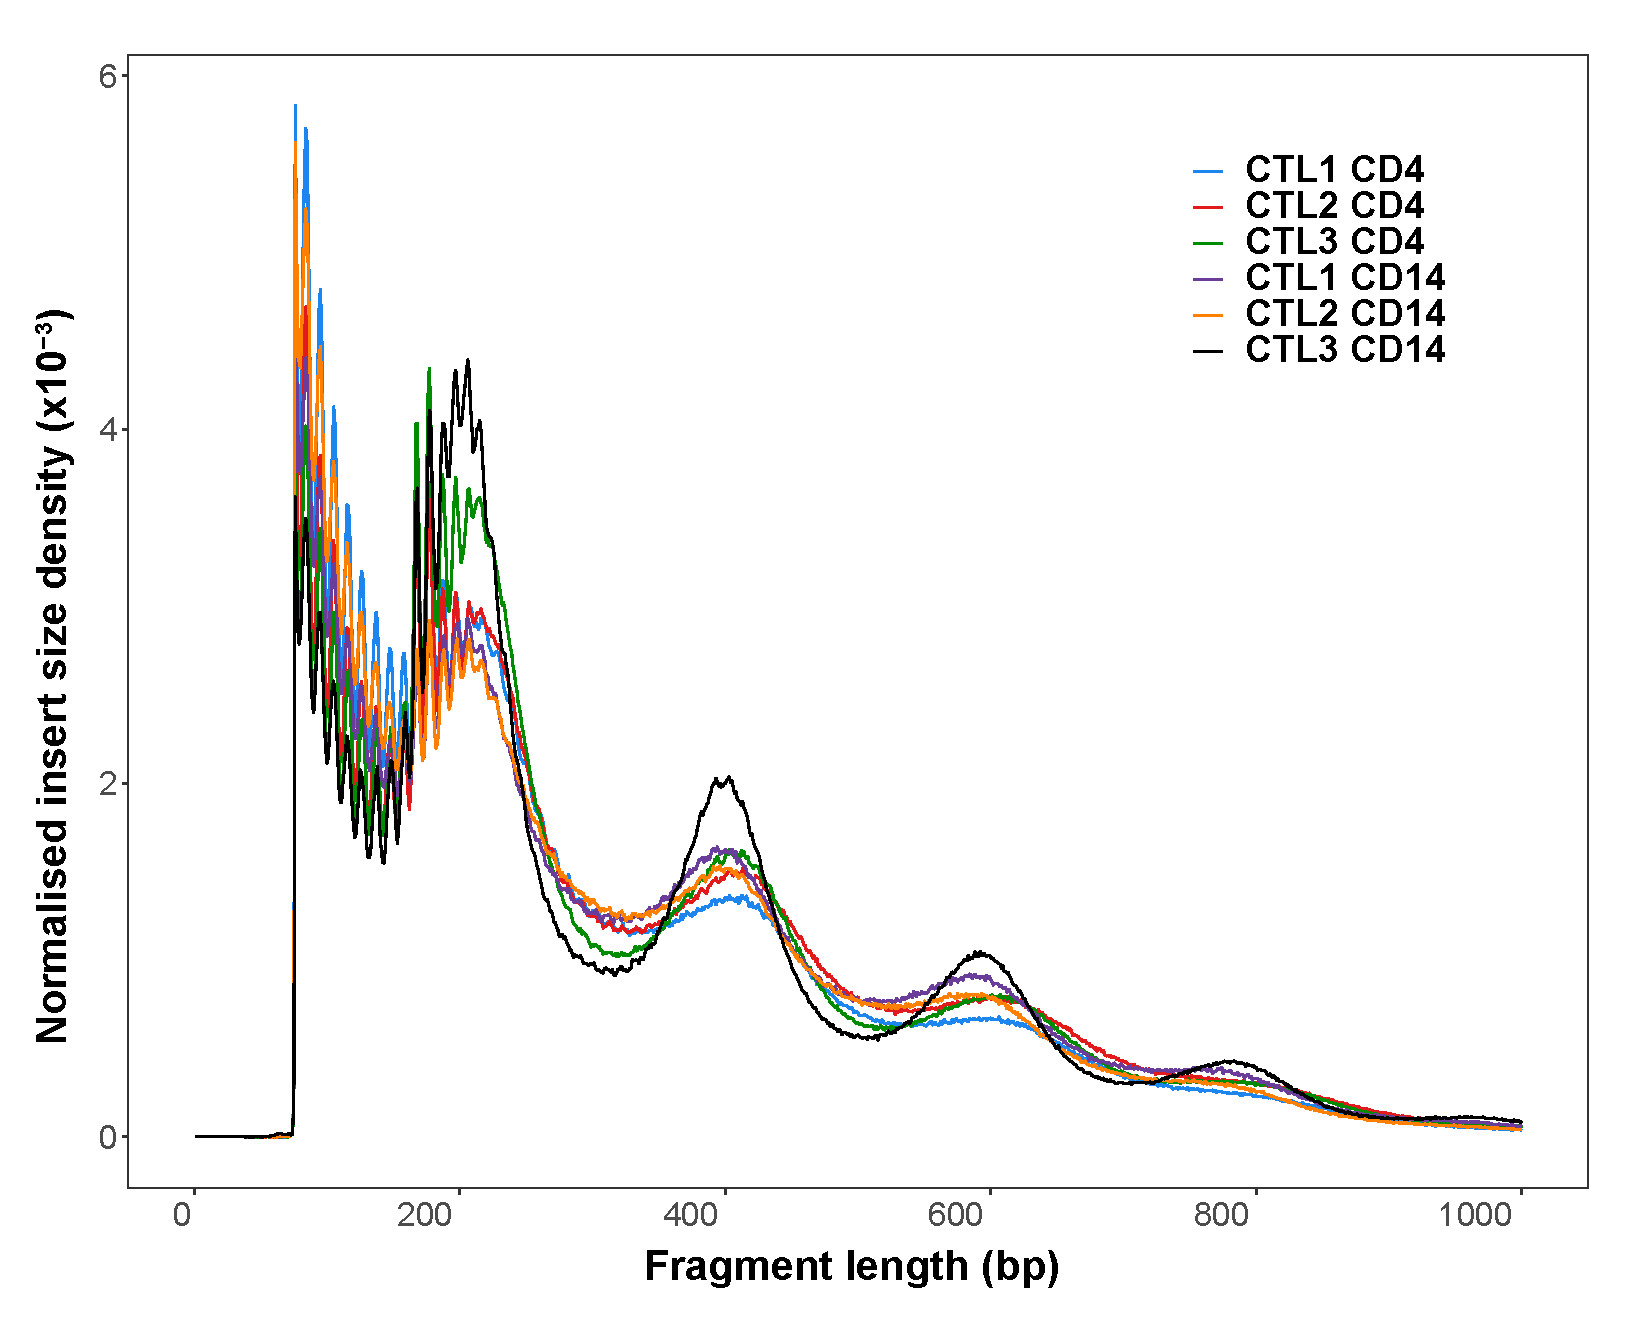
\includegraphics[width=\textwidth]{./Results1/pdfs/ATAC_Core_fresh_CD4_CD14_frag_size_distribution}
\caption{\textbf{A}}
\end{subfigure} %
\begin{subfigure}{0.45\textwidth}
\centering
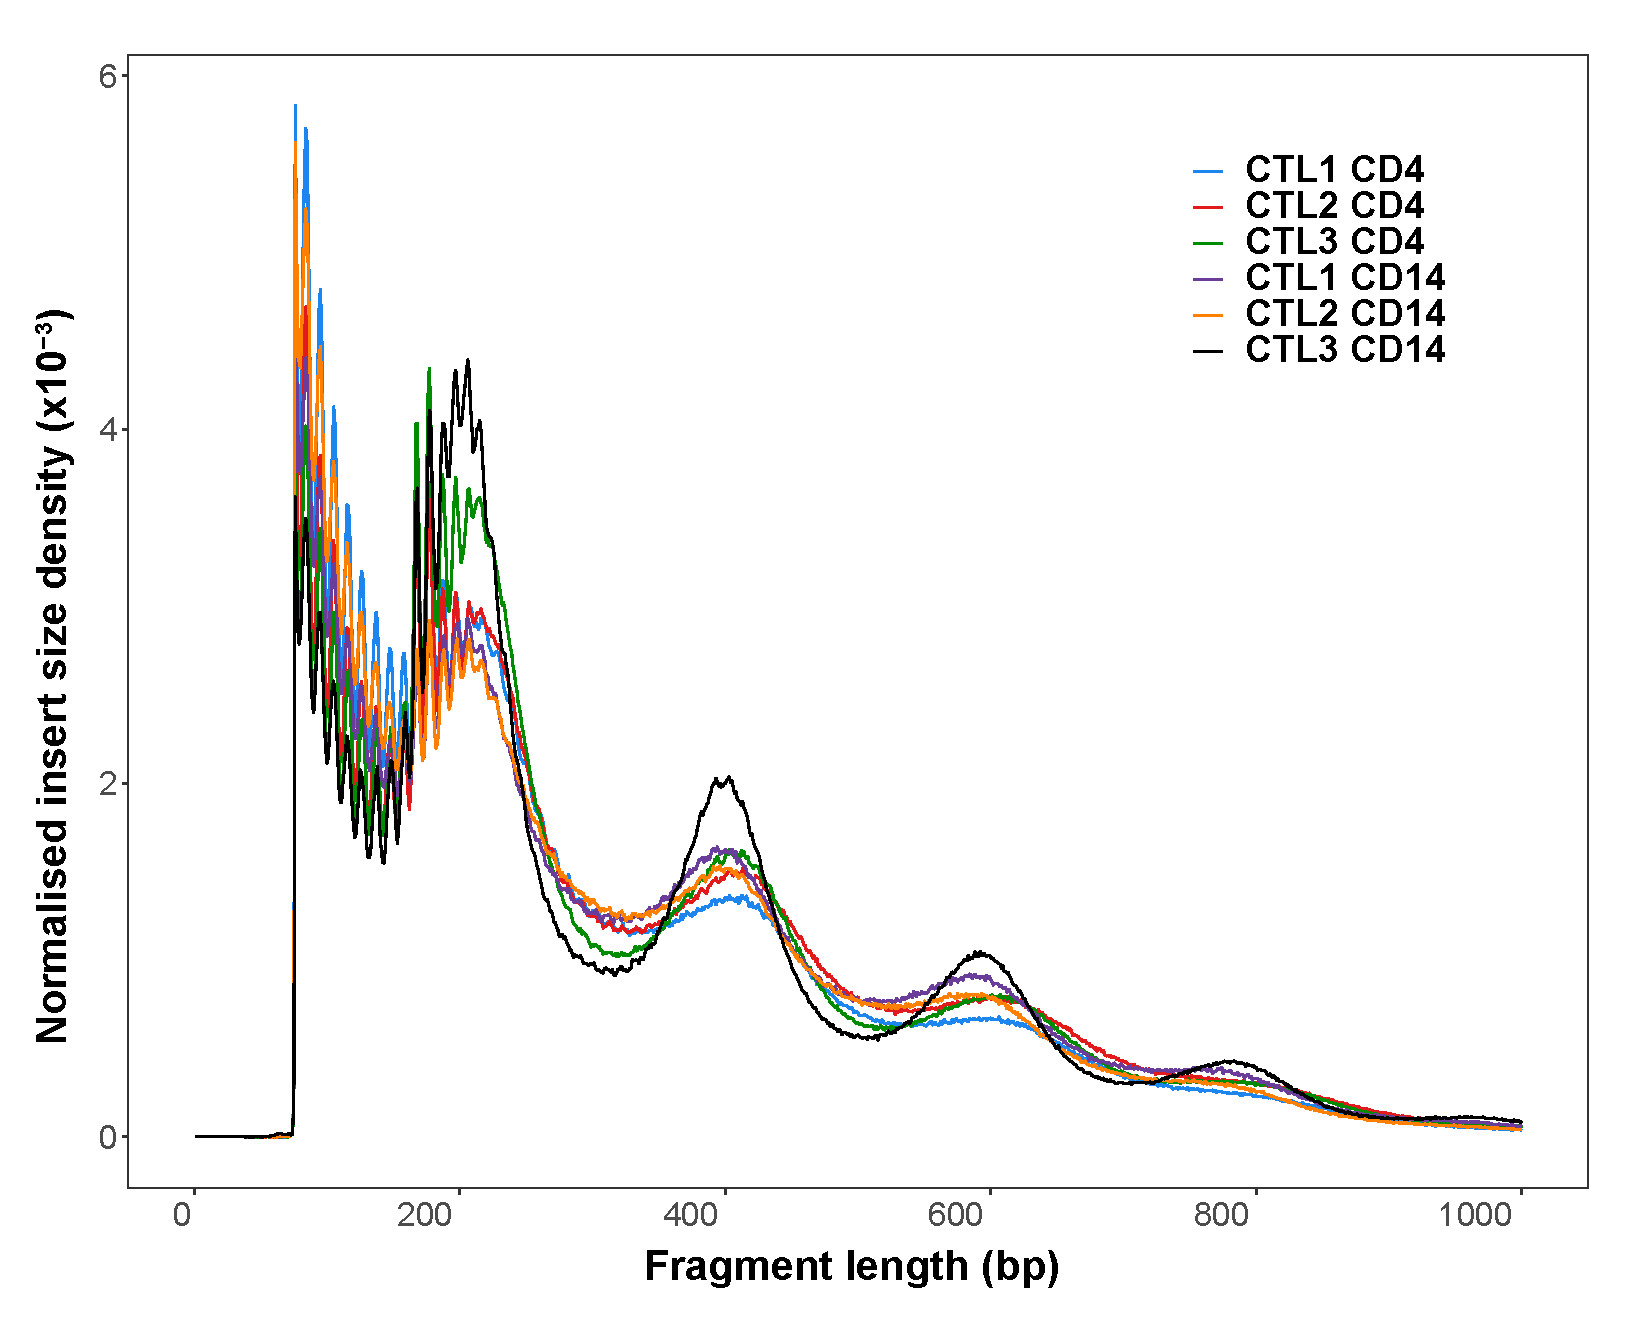
\includegraphics[width=\textwidth]{./Results1/pdfs/ATAC_Core_fresh_CD4_CD14_frag_size_distribution}
\caption{\textbf{B}}
\end{subfigure}

\begin{subfigure}{0.45\textwidth}
\centering
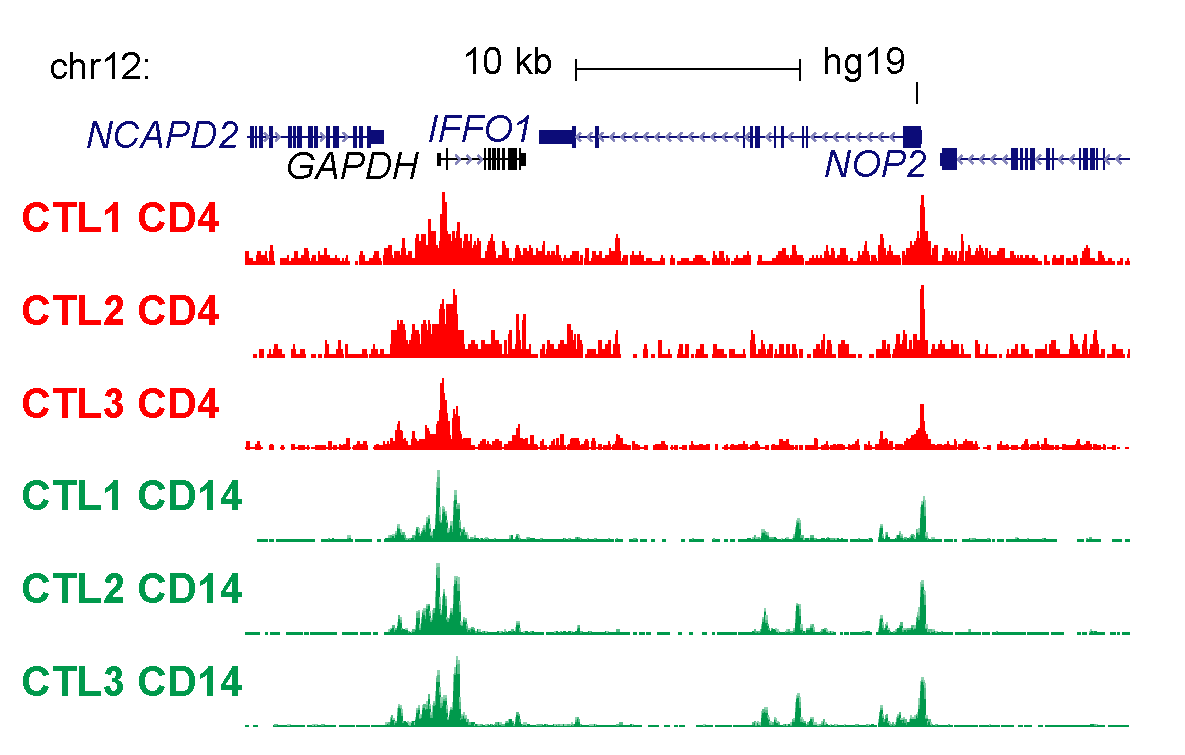
\includegraphics[width=\textwidth]{./Results1/pdfs/ATAC_Core_CD4_CD14_fresh_GAPDH}
\caption{\textbf{C}}
\end{subfigure}

\caption[Measurements for quality control assessment in ATAC-seq samples]{\textbf{} \\
}
\label{fig:QC_ATAC}
\end{figure}
	
The fraction of reads mapping to the location of peaks following basic filtering for FDR<0.01 was calculated for each of the samples using data for 30M reads and a clear positive correlation was found with the TSS enrichment values. 
	
Table for fraction of reads in peaks and \% of mitochondrial reads range between 14.9-43.3\% and they appear to be higher in CD4 than in CD14, opposite to the trend observed for the enrichment of signal at TSS and the fraction of reads in called peaks. Therefore, the percentage of MT reads seems to be cell type dependent and not being directly related with quality sample.
	
\begin{table}[htbp]
%\setlength{\tabcolsep}{20pt} only to stretch the columns if you want
%\renewcommand{\arraystretch}{1.5}
\begin{tabular}{@{} c c c}
\toprule
\textbf{Sample} & \textbf{\% MT reads} & \textbf{Fraction of reads in peaks} \\
\midrule
\midrule
CTL1 CD4 & 14.9 & 4.9 \\
CTL2 CD4 & 30.5 & 5.6 \\
CTL3 CD4 & 28.8 & 7.7 \\
CTL1 CD14 & 43.3 & 24.2 \\
CTL2 CD14 & 36.8 & 28.5 \\
CTL3 CD14 & 37.6 & 24.9 \\
\bottomrule
\end{tabular}
\medskip %gap
\caption[ATAC-seq percentage of MT reads and fraction of reads in called peaks]{\textbf{Details regarding target molecule, fluorochrome, clone, supplier and dilution used for PBMC and SFC staining are provided for each of the antibodies in the panel. In controls only CD3, CD4 and CD4 markers were used.}}
\label{tab:ATAC_MT_fraction_reads_in_peaks}
\end{table}
\bigskip %bigger space

	
	
	
	
	
\begin{landscape}
\begin{table}[htbp]
\setlength{\tabcolsep}{20pt}
%\renewcommand{\arraystretch}{1.5} makes it longer
\begin{center}
\begin{tabular}{@{} c c}
\toprule
\textbf{Publication} & \textbf{Peak calling and filtering} & \textbf{Master list} & \textbf{Differential analysis} \\
\midrule
\midrule
Corces \textit{et al.,}2016 & MACS2 --nomodel  & Rank peak summits -log10pval & ??Quantile normalisation of count matrix\\
                          & Peak summit extension +/-250bp 									& Non overlapping peaks maximally significant & In-house Pearson correlation method\\
\midrule
ENCODE 										& MACS2 --nomodel  								& All IDR significant peaks & Not established\\
                          & Pseudorreplicates IDR analysis 	&  													& \\
													& Only peaks with IDR X 					&  													& \\

\midrule
Matthias 									& MACS2 --nomodel  								& All IDR significant peaks & Not established\\
                          & Pseudorreplicates IDR analysis 	&  													& \\
													& Only peaks with IDR X 					&  													& \\


\midrule
Alasoo \textit{et al.,}2017 & MACS2 --nomodel  								& All IDR significant peaks & Not established\\
														& Pseudorreplicates IDR analysis 	&  													& \\
														& Only peaks with IDR X 					&  													& \\


\midrule
Qu \textit{et al.,}2017 		& MACS2 --nomodel  									& All IDR significant peaks & Not established\\
														& Pseudorreplicates IDR analysis 		&  													& \\
														& Only peaks with IDR X 						&  													& \\

Rendeiro \textit{et al.,}2016 & MACS2 --nomodel  								& All IDR significant peaks & Not established\\
															& Pseudorreplicates IDR analysis 	&  													& \\
															& Only peaks with IDR X 					&  													& \\													
\bottomrule
\end{tabular}
\medskip %gap
\caption[Summary table of ATAC-seq methodology analysis for peak calling, filtering and differential analysis]{\textbf{.}}
\label{tab:ATAC_comparative_methods}
\end{center}
\end{table}
\end{landscape}
\bigskip %bigger space

